\documentclass[a4paper,12pt]{book}
\usepackage[utf8]{inputenc}
\title{}
\author{Rachel Morris}
\date{\today}

\usepackage{rachwidgets}
\usepackage{fancyhdr}
\usepackage{lastpage}
\usepackage{dirtree}
\usepackage{boxedminipage}

\setcounter{chapter}{7}
\setcounter{section}{0}
\newcommand{\laChapter}{7.1 Graph Theory\ }

\newcommand{\laClass}{CS 211\ }
\newcommand{\laSemester}{Fall 2017\ }
\newcounter{question}

\pagestyle{fancy}
\fancyhf{}
\lhead{CS 211 Exercise}
\chead{Fall 2017}
\rhead{Ch \laChapter}
\rfoot{\thepage\ of \pageref{LastPage}}
\lfoot{\scriptsize Compiled by Rachel Morris, last updated \today}

\renewcommand{\headrulewidth}{2pt}
\renewcommand{\footrulewidth}{1pt}

\begin{document}

    %\toggletrue{answerkey}
    \togglefalse{answerkey}
    
    \section{Graph Theory}

    \subsection{The Seven Bridges of K{\"o}nigsberg}

    \begin{quote}
    ``Euler was a Swiss mathematician, physicist, astronomer, logician and engineer who made important and influential discoveries in many branches of mathematics like infinitesimal calculus and graph theory"

    \footnotesize From Wikipedia, https://en.wikipedia.org/wiki/Euler
    \end{quote}

    \begin{center}
        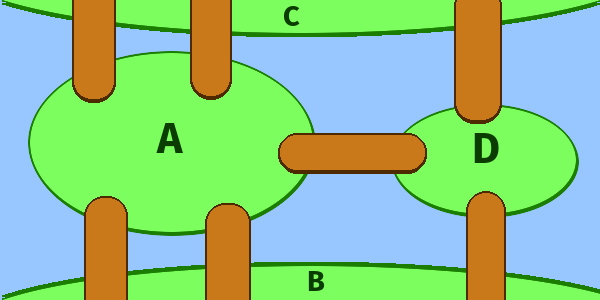
\includegraphics[width=13cm]{images/islands.png}
    \end{center}

    Euler had tried to come up with a solution for whether you could walk over seven bridges in K{\"o}nigsberg, as drawn above,
    exactly once each. To do so, he came up with a graph to model the problem with.

    \begin{center}
        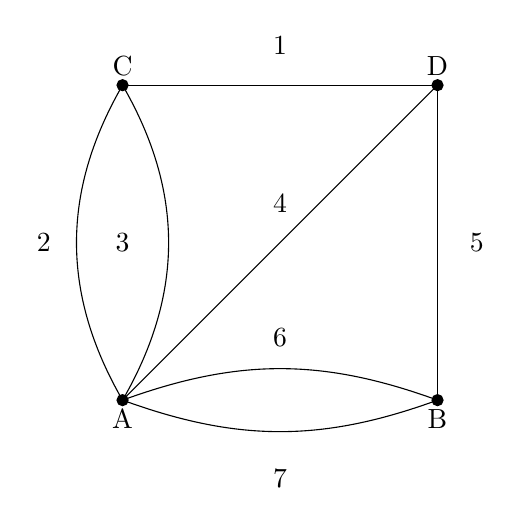
\begin{tikzpicture}
            \filldraw (-2,-2) circle (2pt) node[align=left, below] {A};
            \filldraw (2,-2) circle (2pt) node[align=left, below] {B};
            \filldraw (2,2) circle (2pt) node[align=left, above] {D};
            \filldraw (-2,2) circle (2pt) node[align=left, above] {C};

            \draw (-2,-2)   to (2,2);
            \draw (-2,2)    to (2,2);
            \draw (2,2)     to (2,-2);
            \draw (-2,-2)   to[bend left] (-2,2);
            \draw (-2,-2)   to[bend right] (-2,2);
            \draw (-2,-2)   to[bend left=-20] (2, -2);
            \draw (-2,-2)   to[bend left=20] (2, -2);
            
            \node [fill=none] at (-3, 0) {2};
            \node [fill=none] at (-2, 0) {3};
            \node [fill=none] at (0, 2.5) {1};
            \node [fill=none] at (0, 0.5) {4};
            \node [fill=none] at (2.5, 0) {5};
            \node [fill=none] at (0, -1.2) {6};
            \node [fill=none] at (0, -3) {7};
        \end{tikzpicture}
    \end{center}
    
    

\end{document}
